
\begin{frame}
\frametitle{GRASS: Geographic Resources Analysis Support System}
\begin{itemize}
\item Разрабатывается с 1984 года (USA-CERL). Все это время была открытой ГИС.
\item Кроссплатформенная: доступны версии для GNU/Linux, MS-Windows, Mac OSX, SUN, \dots; 32/64 битные системы.
\item Хорошо документирована, большие коллекции данных. Коммерческая поддержка.
\item Русское зеркало: \href{http://grass.gis-lab.info/index.php}{http://grass.gis-lab.info/index.php}
\end{itemize}
\begin{figure}[!ht]
          \begin{center}
            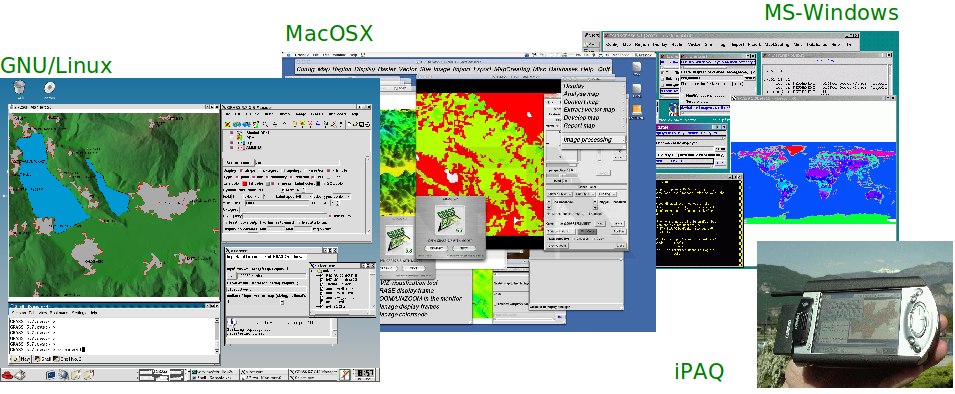
\includegraphics[width=0.8\columnwidth]{./grass/img/platforms.png}
        \end{center}
\end{figure}
\end{frame}

\begin{frame}
\frametitle{GRASS GIS это:}
\begin{multicols}{2}
\begin{itemize}
\item Растровая 2.5D/3D ГИС
\item  Вектроная 2D/3D топологическая ГИС
\item Анализ и обработка графов
\item Система обработки изображений
\item Система 2D и 3D визуализации
\item Поддержка баз данных:dbf, PostgreSQL, MySQL и sqlite. MS SQL, Oracle (ODBC)
\item Поддерживает все распространенные растровые и векторные форматы
\end{itemize}
\begin{figure}[!ht]
          \begin{center}
            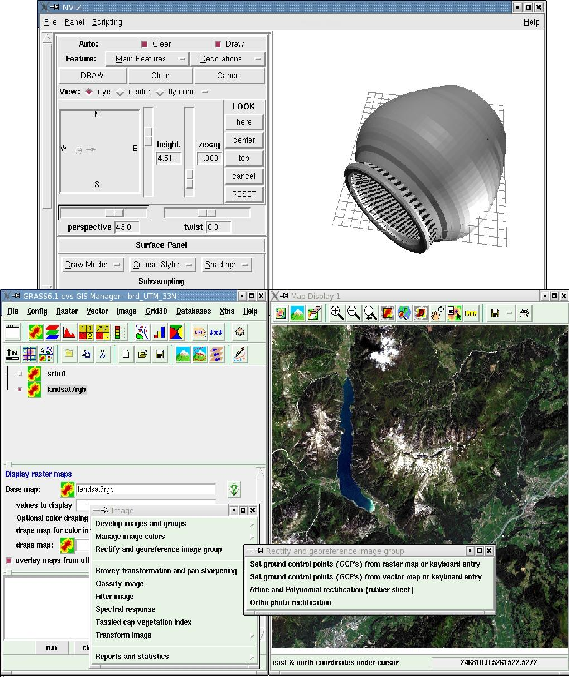
\includegraphics[width=\columnwidth]{./grass/img/views.png}
        \end{center}
\end{figure}
\end{multicols}
\end{frame}


\begin{frame}
\frametitle{Типы пространственных данных}
\begin{itemize}
\item 2D Растровые данные, включая спутниковые снимки и аэрофотосъемку
\item 3D (Voxel) данные
\item  2D/3D векторные данные с поддержкой топологии
\end{itemize}
\begin{figure}[!ht]
          \begin{center}
            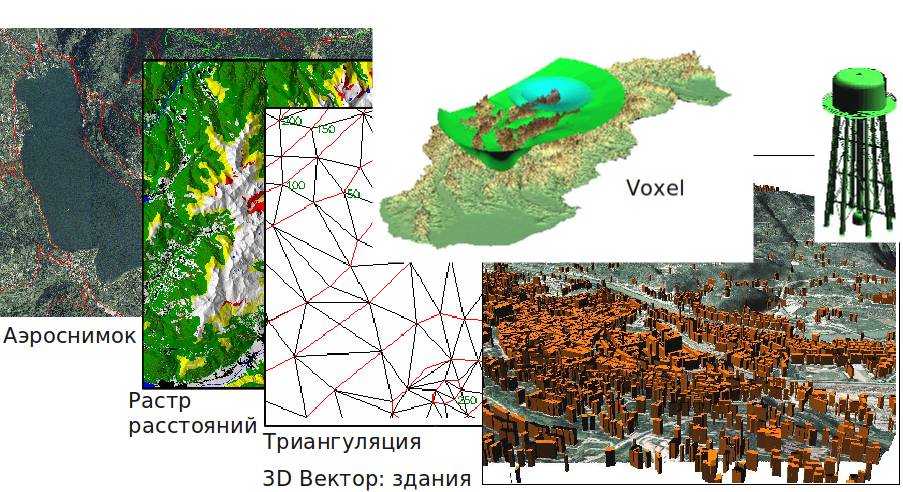
\includegraphics[width=0.8\columnwidth]{./grass/img/datatypes.png}
        \end{center}
\end{figure}
\end{frame}

\begin{frame}
\frametitle{Растровые данные}
\begin{itemize}
\item Растровые данные: представляют собой сетку пикселей, содержащих некоторые значения какого-либо параметра (высота, концентрация и т.п.).
\item Воксельные данные: обобщение растра, переход к трем измерениям.
\end{itemize}
\begin{multicols}{2}
\begin{figure}[!ht]
          \begin{center}
            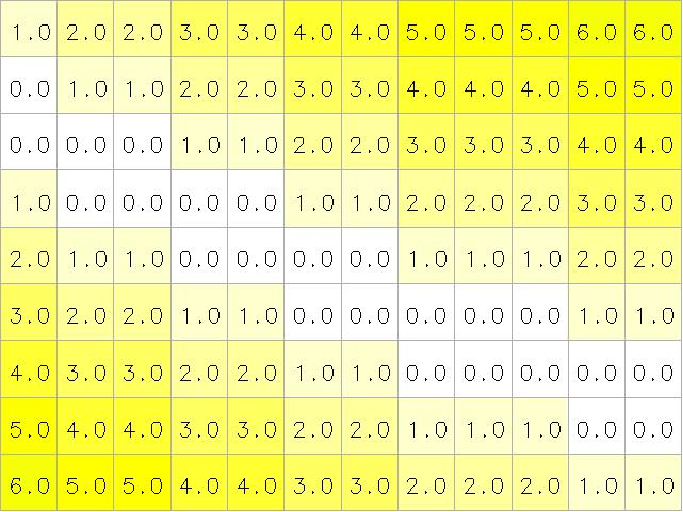
\includegraphics[width=\columnwidth]{./grass/img/raster_model.png}
        \end{center}
\end{figure}
\begin{figure}[!ht]
          \begin{center}
            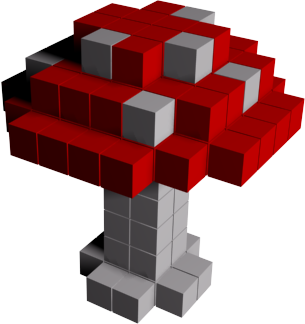
\includegraphics[width=0.7\columnwidth]{./grass/img/voxel_model.png}
        \end{center}
\end{figure}
\end{multicols}
\end{frame}

\begin{frame}
\frametitle{Векторные данные}
\begin{figure}[!ht]
          \begin{center}
            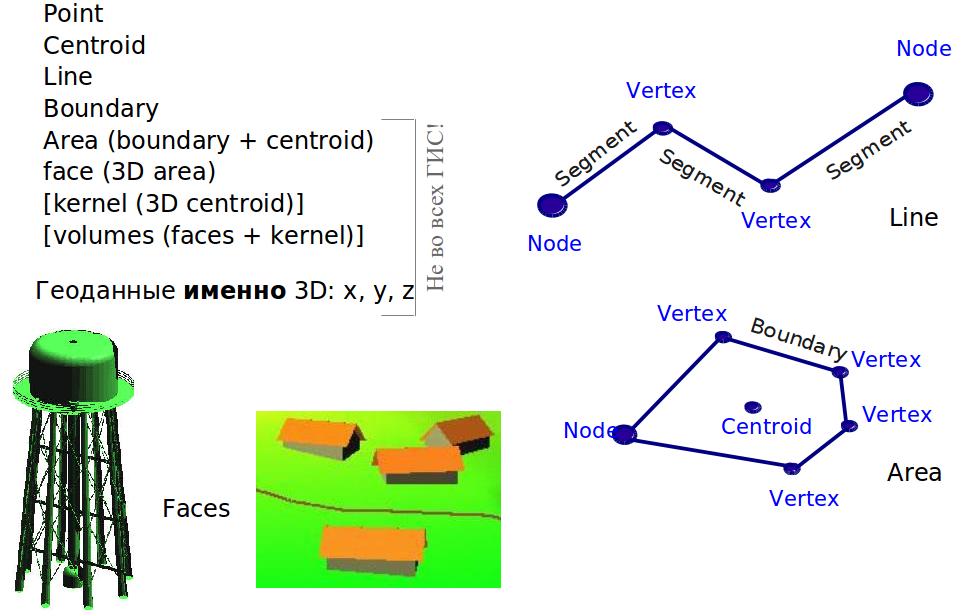
\includegraphics[width=\columnwidth]{./grass/img/vector_data.png}
        \end{center}
\end{figure}
\end{frame}


\begin{frame}
\frametitle{Взаимодействие с другими программами/системами}
\begin{figure}[!ht]
          \begin{center}
            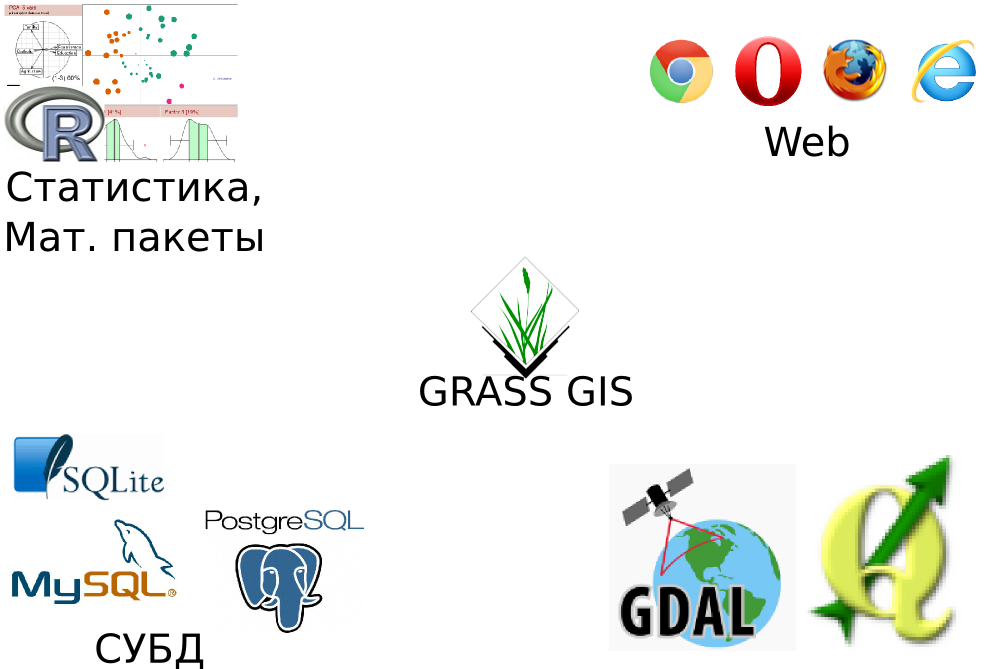
\includegraphics[width=0.9\columnwidth]{./grass/img/grass_prog.png}
        \end{center}
\end{figure}
\end{frame}

